\chapter{Experimental Setup}\label{chapter:second_real_chapter}

\section{Implementation details}
\subsection{Dataset}
\paragraph{COCO\cite{lin2015microsoftcococommonobjects}} is a publicly available dataset and has a multitude of labels. The semantic mask are extrated from the 2017 Panoptic annotations. This set contains more then 100k images that are densly annotated with both the semantic class and instance. There are a total of 133 different classes which belong to 27 'supercategories'. The four categories, "food" and "food-stuff", and "furniture" and "furniture-stuff", were merged into "food" and "furniture" respectively. Bringing the total amount of supercategories to 25. To speed up convergences, we will use these 25 classes. The distribution of the class labels can be seen in Figure \ref{fig:coco-class-distribution}. Some samples of the dataset can be seen in Figure \ref{fig:coco-samples}. More samples can be found in Appendix \ref{appendix:coco_samples}. 

\begin{figure}[h]
    \centering
    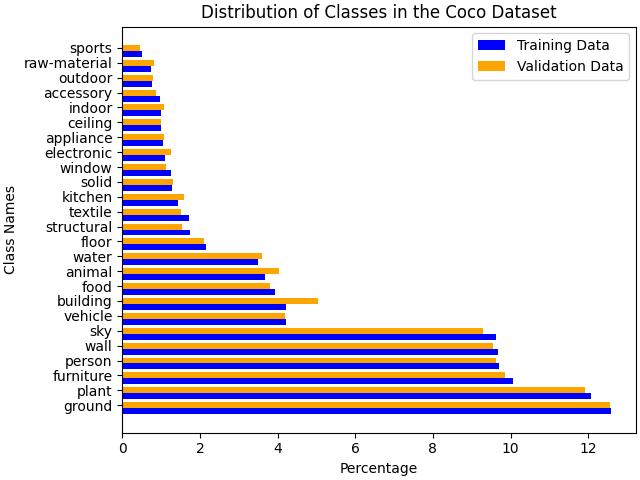
\includegraphics[width=0.9\textwidth]{figures/datasets/coco/class_distribution.png}
    \caption{Class Distribution of CoCo}
    \label{fig:coco-class-distribution}
\end{figure}

\begin{figure}
    \centering
    \subfloat[Training sample 0]{%
        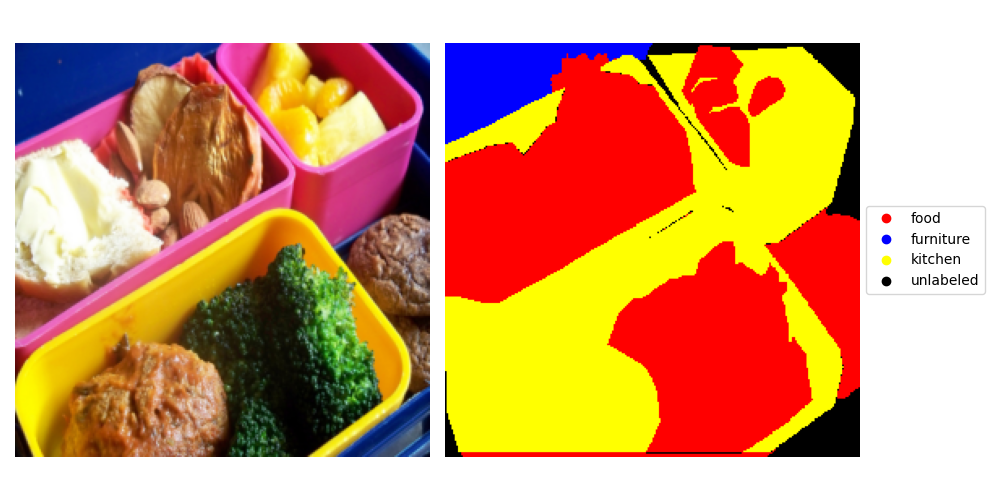
\includegraphics[width=0.5\textwidth]{figures/datasets/coco/samples/train/0.png}%
    }
    \subfloat[Training sample 1]{%
        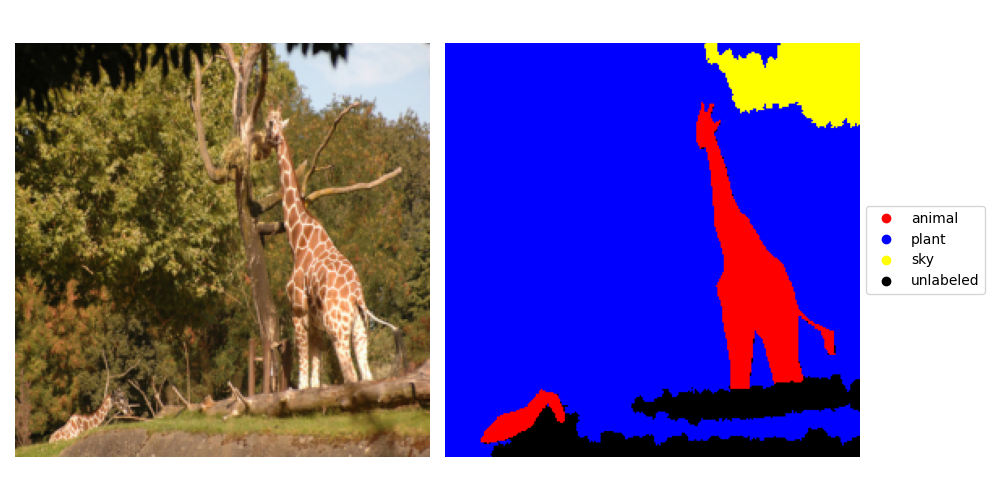
\includegraphics[width=0.5\textwidth]{figures/datasets/coco/samples/train/1.png}%
    }\\
    \subfloat[Validation sample 0]{%
        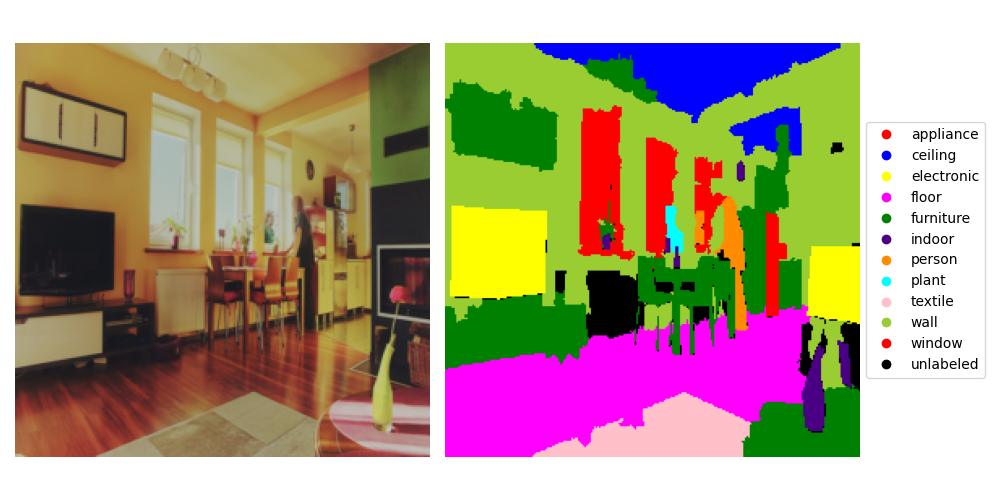
\includegraphics[width=0.5\textwidth]{figures/datasets/coco/samples/val/0.png}%
    }
    \subfloat[Validation sample 1]{%
        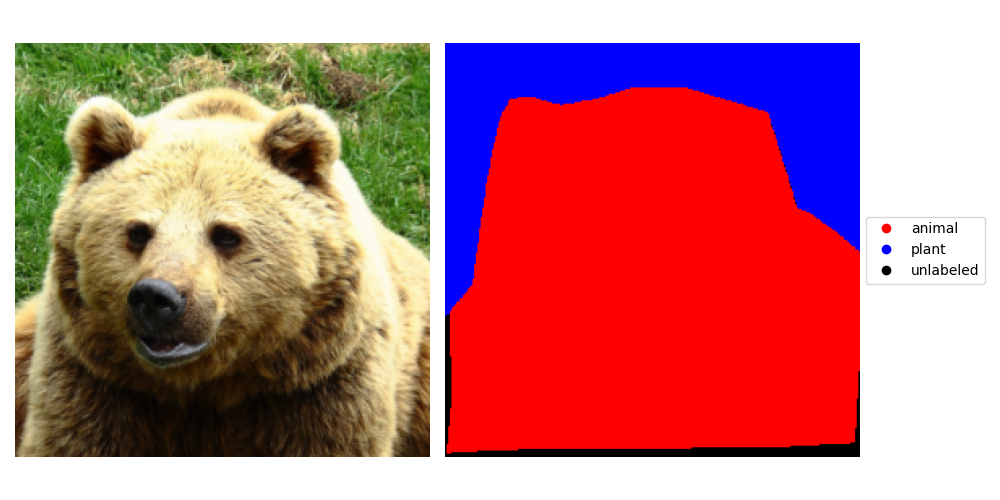
\includegraphics[width=0.5\textwidth]{figures/datasets/coco/samples/val/1.png}%
    }
    \caption{\label{fig:coco-samples}Ground truths for the dataset samples}
\end{figure}


\subsection{Training Settings}
All models are implemented in PyTorch \cite{Ansel_PyTorch_2_Faster_2024} using an adapted version of the segmentation models repository \cite{Iakubovskii:2019}. All code and configs required to train the models and reproduce the experiments can be found on github \footnote[1]{\url{https://github.com/Generative-AI-TUe/msc-project-1297333}}. All models are trained on a NVIDIA Geforce RTX 2080 TI. The gradients are clipped using the norm, with a max value of 10. The AdaMax\cite{kingma2017adammethodstochasticoptimization} is used with a cosine annealing learning rate, varying between $1e^{-3}$ and $1e^-4$. Each model is trained on 10.000 minibatches of size 128, unless otherwise specified.


\section{Is pretraining beneficial}\todo{Not all runs are finished yet}
Each model was trained eight times. Either using no pretrained encoder weights, in the tables referred to as 'None'. Or using pretrained weights retreived from either ImageNet \cite{deng2009imagenet} or a $\beta$-vae. The $\beta$ used for pretraining is added to the weights name. Furthermore, the model is trained twice, once with the frozen (i.e. the encoder weights are not updated) and once where it is finetuned. The resulting Evaluation Jaccard Index can be seen in Table~\ref{tab:baseline_results}.

\begin{table}[ht]
\centering
\caption{The Evaluation Jaccard Index for our model and the baselines for various parameters. The higher the score, the better.}
\label{tab:baseline_results}
\begin{tabular}{llrrrr}
\toprule
 & weights & None & imagenet & vae-b1 & vae-b100 \\
frozen & architecture &  &  &  &  \\
\midrule
\multirow[t]{3}{*}{False} & VAES & 0.21 & 0.47 & 0.20 & 0.15 \\
 & fpn & \textbf{0.30} & \textbf{0.52} & \textbf{0.26} & \textbf{0.28} \\
 & unet & 0.23 & 0.49 & 0.21 & 0.24 \\
\cline{1-6}
\multirow[t]{3}{*}{True} & VAES & n.a. & 0.40 & 0.20 & 0.18 \\
 & fpn & n.a. & 0.45 & 0.21 & 0.21 \\
 & unet & n.a. & 0.42 & 0.20 & 0.19 \\
\cline{1-6}
\bottomrule
\end{tabular}
\end{table}


\todo{TODO: Run statistical analysis on resutls.}
\begin{itemize}
    \item Compare {all}-vae1-frozen to {all}-img-frozen
    \item Compare {all}-vae1-unfrozen to {all}-{rand, img}-unfrozen
\end{itemize}

Include the current image
\begin{figure}[h]
    \foreach \i in {0,1,...,4} {
            \centering
            \subfloat[Image]{\includegraphics[width=0.2\textwidth]{figures/baselines/samples/VAES-imagenet-False/\i.png}}
            \subfloat[Ground Truth]{\includegraphics[width=0.2\textwidth]{figures/baselines/samples/VAES-imagenet-False/gt_\i.png}}
            \subfloat[VAES-imagenet]{\includegraphics[width=0.2\textwidth]{figures/baselines/samples/VAES-imagenet-False/pr_\i.png}}
            \subfloat[unet-imagenet]{\includegraphics[width=0.2\textwidth]{figures/baselines/samples/unet-imagenet-False/pr_\i.png}}
            \subfloat[fpn-imagenet]{\includegraphics[width=0.2\textwidth]{figures/baselines/samples/fpn-imagenet-False/pr_\i.png}}
            \\
        }
    \caption{Samples of the validation dataset, with the ground truth and the prediction by the model. The encoder is not frozen. (Note: FPN Result is not the correct image yet)}\label{ref:baseline-sample-results-0}
\end{figure}


\section{Reduction data required}
To determine if pretraining results in a reduction of labeled training data required, a full factorial design is done over the parameters: architecture type, pretrained weights, and the percentage of the (labeled) dataset used. The resulting Jaccard Index of each combination can be seen in Table~\ref{tab:data_fraction_results} and are plotted in Figure~\ref{fig:dataset-fraction-results}.
\begin{table}[ht]
\centering
\caption{The Evaluation Jaccard Index for the various models and dataset fractions. The higher the score the better.}
\label{tab:data_fraction_results}
\begin{tabular}{llrrrr}
\toprule
 & fraction & 1.000000 & 0.100000 & 0.010000 & 0.001000 \\
architecture & weights &  &  &  &  \\
\midrule
\multirow[c]{3}{*}{VAES} & None & 0.15 & 0.16 & 0.18 & 0.12 \\
 & imagenet & 0.34 & 0.37 & 0.39 & 0.21 \\
 & vae-b10 & 0.14 & 0.16 & 0.18 & 0.12 \\
\multirow[c]{3}{*}{fpn} & None & 0.22 & 0.12 & 0.21 & 0.17 \\
 & imagenet & 0.45 & \textbf{0.48} & \textbf{0.48} & \textbf{0.34} \\
 & vae-b10 & 0.19 & 0.21 & 0.23 & 0.16 \\
\multirow[c]{3}{*}{unet} & None & 0.21 & 0.10 & 0.18 & 0.14 \\
 & imagenet & \textbf{0.46} & 0.44 & 0.43 & 0.30 \\
 & vae-b10 & 0.20 & 0.18 & 0.21 & 0.14 \\
\bottomrule
\end{tabular}
\end{table}


\begin{figure}[h]
    \centering
    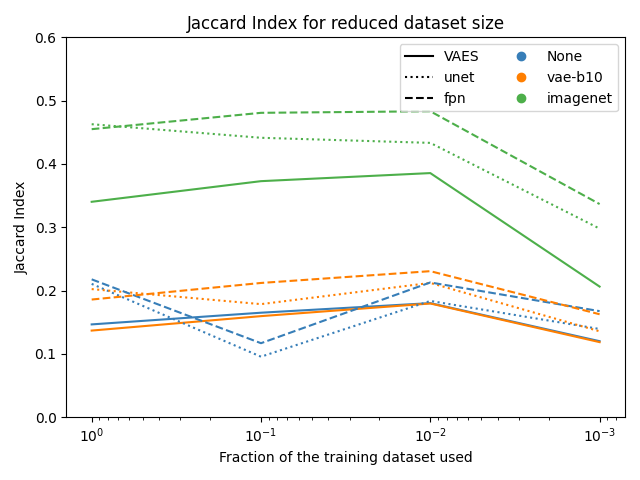
\includegraphics[width=0.9\textwidth]{figures/data_percentage/line-plot.png}
    \caption{Jaccard Index for reduced training dataset size.}
    \label{fig:dataset-fraction-results}
\end{figure}

An Analisyses of Variance (ANOVA) is done, which can be seen in Table~\ref{tab:data_fraction_parameter_significance}. Based on which, it can be determined that there are no significant interaction effects between any of the parameters, and that each individual parameter has a significant effect.
\begin{table}[ht]
\centering
\caption{Anova results estimating the influence of each parameter.\\Where: \\\hphantom{tabb}`weights' are the pretrained weights (or lack thereof) used.\\\hphantom{tabb}`architecture' is the model architecture used.\\\hphantom{tabb}`$\log_{10}(\text{fraction})$' is the fraction of data used in log scale.\\\hphantom{tabb}$A$:$B$ is the interaction effect between $A$ and $B$}
\label{tab:data_fraction_parameter_significance}
\begin{tabular}{lrrrrr}
\toprule
 & df & sum\_sq & mean\_sq & F & PR(>F) \\
\midrule
weights & 2.00 & 0.39 & 0.20 & 75.49 & \textbf{0.00} \\
architecture & 2.00 & 0.02 & 0.01 & 4.61 & \textbf{0.02} \\
weights:architecture & 4.00 & 0.01 & 0.00 & 0.93 & 0.47 \\
$\log_{10}(\text{fraction})$ & 1.00 & 0.02 & 0.02 & 6.45 & \textbf{0.02} \\
$\log_{10}(\text{fraction})$:weights & 2.00 & 0.01 & 0.01 & 2.11 & 0.15 \\
$\log_{10}(\text{fraction})$:architecture & 2.00 & 0.00 & 0.00 & 0.22 & 0.80 \\
$\log_{10}(\text{fraction})$:weights:architecture & 4.00 & 0.00 & 0.00 & 0.01 & 1.00 \\
Residual & 18.00 & 0.05 & 0.00 & n.a. & n.a. \\
\bottomrule
\end{tabular}
\end{table}


The effect of the parameters can then be analyzed using a simple OLS model. The results of which are shown in Table~\ref{tab:data_fraction_parameter_influence}. It shows that there is a large and significant increase in preformance when using the ImageNet weights. The weights gained from pretraining a VAE do not significantly affect the performance, compared to random weights. Furthermore, both the FPN and UNet architectures are better then the VAES architecture. Finally, the size of the dataset is significant, however it is more important to choose the right architecture and especially pretrained weights.
\begin{table}
    \centering
    \caption{Coefficients of the OLS.\\Where:\\\hphantom{tabb}Coef. is the effectsize.\\\hphantom{tabb}P> |t| is the $p$-value. Bolded if significant ($\alpha\leq0.05$).}
    \label{tab:data_fraction_parameter_influence}
    \begin{tabular}{lrrrrrr}
        \toprule
                                     & Coef. & Std.Err. & t     & P>|t|         & [0.025 & 0.975] \\
        \midrule
        Intercept                    & 0.16  & 0.02     & 7.56  & \textbf{0.00} & 0.12   & 0.20   \\
        weights[T.imagenet]          & 0.23  & 0.02     & 11.66 & \textbf{0.00} & 0.19   & 0.27   \\
        weights[T.vae-b10]           & 0.01  & 0.02     & 0.67  & 0.50          & -0.03  & 0.05   \\
        architecture[T.fpn]          & 0.06  & 0.02     & 3.19  & \textbf{0.00} & 0.02   & 0.10   \\
        architecture[T.unet]         & 0.04  & 0.02     & 2.05  & \textbf{0.05} & 0.00   & 0.08   \\
        $\log_{10}(\text{fraction})$ & 0.02  & 0.01     & 2.71  & \textbf{0.01} & 0.00   & 0.03   \\
        \bottomrule
    \end{tabular}
\end{table}



\section{Ablation Study}
\subsection{Influence of the backbone}
We first analyze the influence of the backbone on the performance of the VAE task by comparing the following backbones, MobilenetV2 \cite{sandler2019mobilenetv2invertedresidualslinear}, EfficientNet \cite{tan2020efficientnetrethinkingmodelscaling} and Resnet50 \cite{he2015deep}. The results can be seen in Table \ref{tab:vae-backbones}. Some examples of the reconstruction capabillities can be seen in Figure \ref{fig:vae-backbones}

\begin{table}[!ht]
    \centering
    \caption{Loss values resulting from training a Beta-VAE for various $\beta$ values}
    \label{tab:vae-backbones}
    \begin{tabular}{ccc}
        \hline
        $\beta$ & Kl-Divergence & Reconstruction Error (x1e5) \\
        \hline
        0.01    & 80200         & 1.9                         \\
        0.1     & 31250         & 1.5                         \\
        1       & 8190          & 2.7                         \\
        10      & 2089          & 2.2                         \\
        100     & n.a.          & (node crashed mid run)      \\
        \hline
    \end{tabular}
\end{table}

\begin{figure}[!ht]
    \centering
    \caption{Example reconstruction for a few of the models}
    \label{fig:vae-backbones}
    \subfloat[Original, $\beta$ = 0.01]{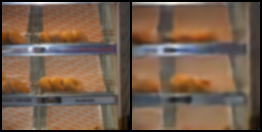
\includegraphics[width=0.45\linewidth]{figures/beta-vae/b0.01-0.png}}
    \subfloat[Original, $\beta$ = 0.1]{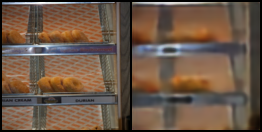
\includegraphics[width=0.45\linewidth]{figures/beta-vae/b0.1-0.png}} \quad
    \subfloat[Original, $\beta$ = 1]{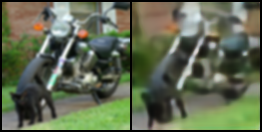
\includegraphics[width=0.45\linewidth]{figures/beta-vae/b1-0.png}}
    \subfloat[Original, $\beta$ = 10]{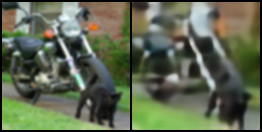
\includegraphics[width=0.45\linewidth]{figures/beta-vae/b10-0.png}}
\end{figure}


\subsection{Influence of the Beta factor}
We also analyze the effect of the beta factor on the reconstruction quality of the vae. This is done by training models with varying values for beta. The results can be seen in Table \ref{tab:beta-vae-loss-values}. Some examples of the reconstruction capabillities can be seen in Figure \ref{fig:beta-vae-recon-examples}.

\begin{table}[!ht]
    \centering
    \caption{Loss values resulting from training a Beta-VAE for various $\beta$ values}
    \label{tab:beta-vae-loss-values}
    \begin{tabular}{ccc}
        \hline
        $\beta$ & Kl-Divergence & Reconstruction Error (x1e5) \\
        \hline
        0.01    & 80200         & 1.9                         \\
        0.1     & 31250         & 1.5                         \\
        1       & 8190          & 2.7                         \\
        10      & 2089          & 2.2                         \\
        100     & 498           & 2.9                         \\
        \hline
    \end{tabular}
\end{table}

\begin{figure}[!ht]
    \centering
    \caption{Example reconstructions for $\beta$-vae.}
    \label{fig:beta-vae-recon-examples}
    \subfloat[Original, $\beta$ = 0.01]{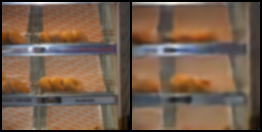
\includegraphics[width=0.45\linewidth]{figures/beta-vae/b0.01-0.png}}
    \subfloat[Original, $\beta$ = 0.1]{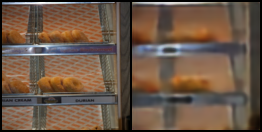
\includegraphics[width=0.45\linewidth]{figures/beta-vae/b0.1-0.png}} \quad
    \subfloat[Original, $\beta$ = 1]{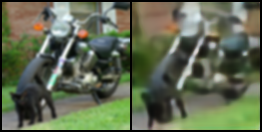
\includegraphics[width=0.45\linewidth]{figures/beta-vae/b1-0.png}}
    \subfloat[Original, $\beta$ = 10]{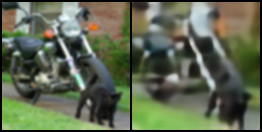
\includegraphics[width=0.45\linewidth]{figures/beta-vae/b10-0.png}}
\end{figure}


\subsection{Skip Connection}
To understand the importance of the skip connections which are added after the pretraining. We will show the effect of this by incrementally removing more skip connections.
\todo{Training is in the backlog of slurm}

\begin{table}[!ht]
    \centering
    \caption{Results when removing skip connections.}
    \label{tab:abl-skip-connection}
    \begin{tabular}{cccc}
        \hline
        Num Skip Connections & CrossLoss (x1e6) & Eval JI & Train JI \\
        \hline
        0 (Only midblock)    & n.a.             & n.a.    & n.a.     \\
        1                    & n.a.             & n.a.    & n.a.     \\
        2                    & n.a.             & n.a.    & n.a.     \\
        3                    & n.a.             & n.a.    & n.a.     \\
        4                    & n.a.             & n.a.    & n.a.     \\
        5 (all)              & n.a.             & n.a.    & n.a.     \\
        \hline
    \end{tabular}
\end{table}
